\newpage
\subsection{Parasitic elements}
\label{sec:parasitic}

Many devices have parasitic shunt and series resistances associated with them.  Shunt resistances ($R_{s}$) are caused by conduction straight through the device in thin novel devices this is often caused by impurities in the material system.  Parasitic series resistances ($R_{s}$) are often associated with the resistance of the contacts, the resistance of the HTL/ETL or any other resistances which are not associated with the active layer.  These resistance can be seen for a typical solar cell in figure \ref{fig:parasitic_circuit} also shown in the figure is the ideal diode of the device. These resistances can be set in the parasitic component window shown in figure \ref{fig:parasitic}
\\
\\
\noindent
\begin{minipage}{0.45\textwidth}
\centering
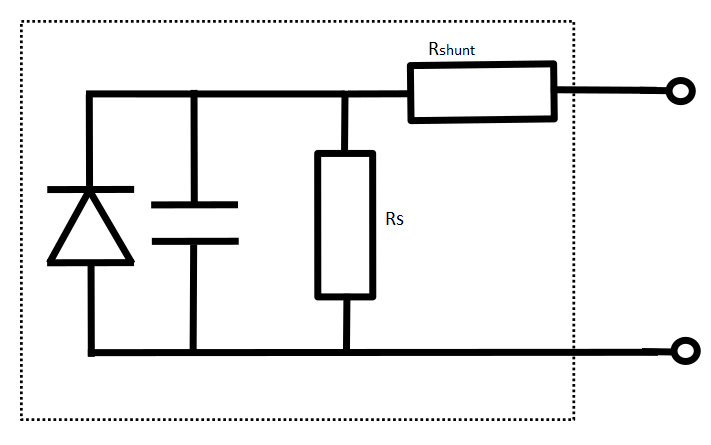
\includegraphics[width=\textwidth,height=0.7\textwidth]{./images/running/parasitic_circuit.png}
\captionof{figure}{Circuit model of a solar cell.}
\label{fig:parasitic_circuit}
\end{minipage}
\hspace*{10px}
\begin{minipage}[]{0.45\linewidth}
\centering
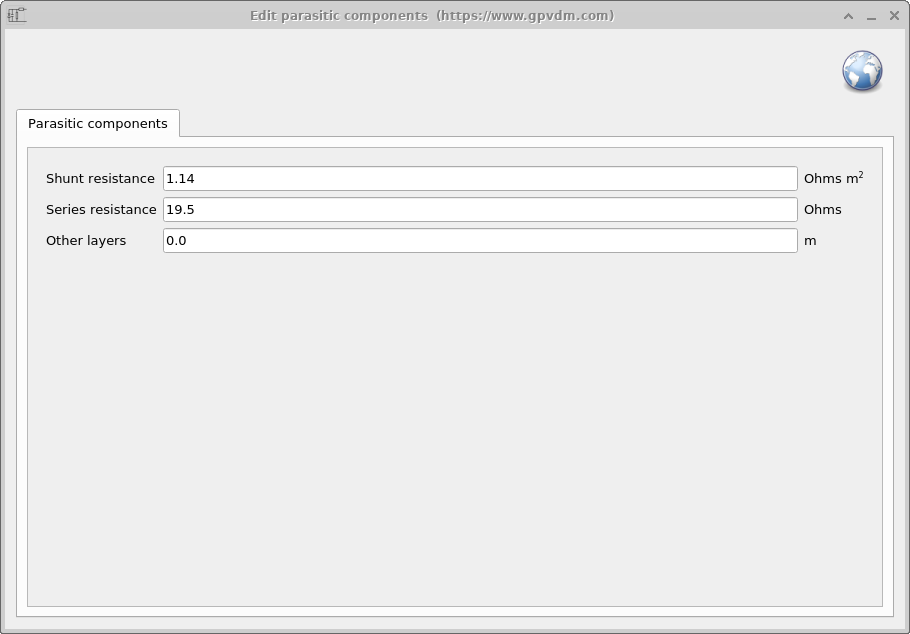
\includegraphics[width=\textwidth,height=0.7\textwidth]{./images/running/parasitic.png}
\captionof{figure}{The parasitic component editor.}
\label{fig:parasitic}
\end{minipage}


You can change the values of series and shunt resistance in OghmaNano, by going to the \emph{Electrical} tab and then clicking on the \emph{Parasitic components} button. Due to the flat broad contacts on a solar cell, there is often a capacitance associated with the device, this is important for transient measurements and can be calculated with the equation:

\begin{equation}
C=\frac{\epsilon_r \epsilon_0 A}{d+\Delta}
\end{equation}

where $A$ is the area of the device $\epsilon$ are the hyperactivities, and $d$ is the thickness of the device.  Often for various reasons the measured capacitance of the device does not match what one would expect from the above equation. Therefore the term "Other layers" ($\Delta$) has been added to the parasitic window to account for differences between measured capacitance and layer measured layer thicknesses.

\vspace*{\fill}
\fbox{
\parbox{0.9\textwidth}{
\color{blue} Task \addtocounter{question}{1}\thequestion : In the optical tab you will find a control called \emph{Light intensity}, this controls the amount of light which falls on the device in Suns.  Set it to zero so that the device is in the dark.  Then run two JV curve simulations, one with a shunt resistance of $1~Ohm~m^2$ and one with a shunt resistance of $1x10^{6}~Ohm~m^2$ (Hint you will have to enter $1e6$ in the text box).  What happens to the dark JV curve?  Now try running the same same simulations again but in the light.
}\par
}


